\section{Introduction}

In the setting of modern data centers and HPC clusters, there have been numerous research efforts
to enhance performance. Data Analytics applications that rely on machine and deep learning techniques demand
tremendous workloads with their need for massive computing performance, and have led to the wide adoption of graphics
processing units (GPU) accelerator and multicore (CPU) technologies, which are pushing current datacenter interconnect
and memory architectures to their limit\cite{shalf19}.

Furthermore, communication using conventional ethernet fabric is a severe inhibitor to efficient resource sharing.
For emerging compute intensive and resource hungry applications, substantial increases in bandwidth are a necessity\cite{shalf19}.

A shift towards high speed network fabrics has been proven useful,
because it helps alleviaite the latencies that may arise from node to node communication.
The usage of InfiniBand fabrics over Ethernet fabrics is common in such setting.

The amount of time that a processor is engaged in the transmition or reception of a message, also known as overhead,
can also play a major role in performance, since the processor cannot perform other operations.
This is especially true for applications that are heavy on read/write operations, as they can
be slowed down significantly by high oveheads.\cite{martin97}

To tackle this problems, a common solution applied in industry is the usage of InfiniBand, which
is a network architecture which supports Remote Direct Memory Access (RDMA).
RDMA works by letting the Network Interface Card (NIC) and the User Application (more specifically, its memory)
directly communicate with each other, therefore bypassing the Operating System (which is known for
causing high overhead through context switches to kernel space) and thus offloading the CPU. This practice has been
gaining traction in the HPC environment, aiding multiple machines to mitigate bottlenecks and efficiently act like a
single large system.

Taking advantage of the InfiniBand architecture requires specialized hardware, as the InfiniBand network architecture defines
its own protocols for each network layer. Moreover, special NICs, which go by the name of Channel Adapters (CA) in the InfiniBand
architecture are also required. Specifically, A CA is a programmable DMA engine which special protection features that allow
DMA operations to be initated locally and remotely\cite{infinibandvol107}.

As the combination IP/Ethernet is an ubiquitous technology, the need for a similar technology which allows
RDMA without having to resort to specialized hardware arised. RDMA over Converged Ethernet (RoCE) is an modification
to the InfiniBand stack, which replaces the link and physical layers for those of Ethernet,
allowing to use regular switches to provide InfiniBand services. Since  RoCE traffic does not carry an IP header,
it cannot be routed across the boundaries of Ethernet networks using regular IP routers\cite{rocev2}.


The RoCEv2 specification is an extension of the former, it allows routers to transport
IB packets contained within a UDP datagram over the IP protocol. But Nevertheless, RDMA operations still require RoCE adapter
cards as to take the involvement of the OS out of the picture.

An open source software implementation of the RDMA transport, called SoftRoCE, has been part of the mainline tree of
the linux kernel since late 2016. SoftRoCE is implemented as a device driver and it provides a complete RDMA
stack implementation over any regular NIC\cite{softroce}.

\begin{figure}
  \centering
  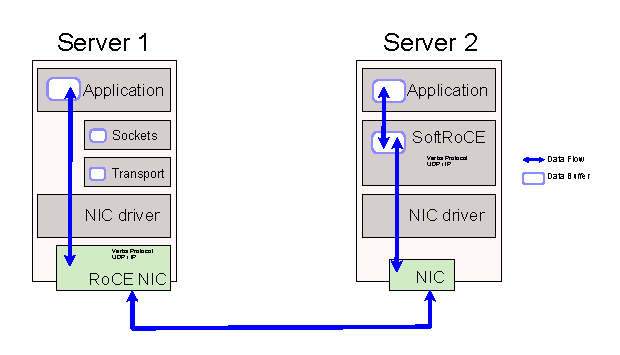
\includegraphics[]{softrocepretty}
  \caption[softroce]{SoftRoCE allows RDMA interaction with RoCE devices\footnotemark}
\end{figure}

\footnotetext{adapted from \url{ https://www.roceinitiative.org/wp-content/uploads/2016/11/SoftRoCE_Paper_FINAL.pdf }}

More importantly, SoftRoCE enables interoperation between a server equipped with a RoCE adapter card, and a server running on
commodity hardware. The fact that any hardware and even VMs can be part of an RDMA architecture, bridges an important gap in the RDMA ecosystem.


%% interops between regular nic and roce nic
%% SoftRoCE software alternative to make RDMA available without HW and even in VMs.
%% https://www.roceinitiative.org/wp-content/uploads/2016/11/SoftRoCE_Paper_FINAL.pdf

\subsection{Task description}

Remote Direct Memory Access (RDMA) networks offer significant performance benefits by exposing the (network) device directly
to the user application. On one hand RDMA-networks remove the operating system from the critical path of 
communication. But on the other hand, the interface from the application to the operating system and from 
the application to the device becomes significantly more complicated. In comparison to traditional sockets-based API, 
such design increases the attack surface of the OS and the underlying network infrastructure.

With the increasing adoption of RDMA-networks in cloud and HPC settings, the attacker models consider user applications 
to be potentially malicious. Therefore, the interface between the application and the RDMA-network must be secure.
The existing works have already shown fundamental problems in state-of-the art RDMA network architectures, but 
have not yet studied the safety of the API itself. The goal of this work is to characterise the attack surface 
created by the RDMA communication API.

The goal of this project is to characterise possible attack vectors coming through the RDMA API. Furthermore, the 
project must propose measures to harden the attack surface. A promising approach for hardening RDMA API is to apply 
fuzzing techniques aimed to find potential vulnerabilities in existing kernel-level RDMA-infrastructure. If such 
direction is chosen, the student shall design a fuzzing infrastructure targeting RDMA devices or RDMA device 
drivers. As such, the fuzzing infrastructure may rely on specifics of RDMA-network architectures to make bug-finding 
more efficient.

\subsection{Goals}

Given the relevance and usefulness of SoftRoCE, it is a major concern for it to be safe and reliable.
Using a software testing technique which has been gaining popularity recently due to its efficiency in
discovering bugs, namely fuzzing, this work aims to explore and describe ways to identify the attack surface
of this particular device driver and the API it exposes.

% One of the focuses of this work is to approach testing the API exposed by a specific device driver, SoftRoCE, which leverages RDMA
% for linux kernels in a systematical fashion.
